\chapter{Evaluation}
\newcommand{\rd}[1]{\textcolor{red}{#1}}
\newcommand{\gn}[1]{\textcolor{green}{#1}}

\label{Chapter5}

in the previous chapter \ref{Chapter4} the test bed implementation was introduced. In this chapter this test bed is used to evaluate the performance of the system proposed in chapter \ref{Chapter3}.

The evaluated components of the system are the room recognition and the room based weighting method for the trilateration.

Before presenting the evaluation results section \ref{TestBedDeployment} introduces the environment where the test bed was deployed and the data sets used for the evaluation. Sections \ref{EvaluationRoomRecognition} and \ref{EvaluationWeighting} then evaluate the room recognition and weighting method.

\section{Test bed deployment and collected data sets}
\label{TestBedDeployment}

\begin{figure}[ht]
\centering
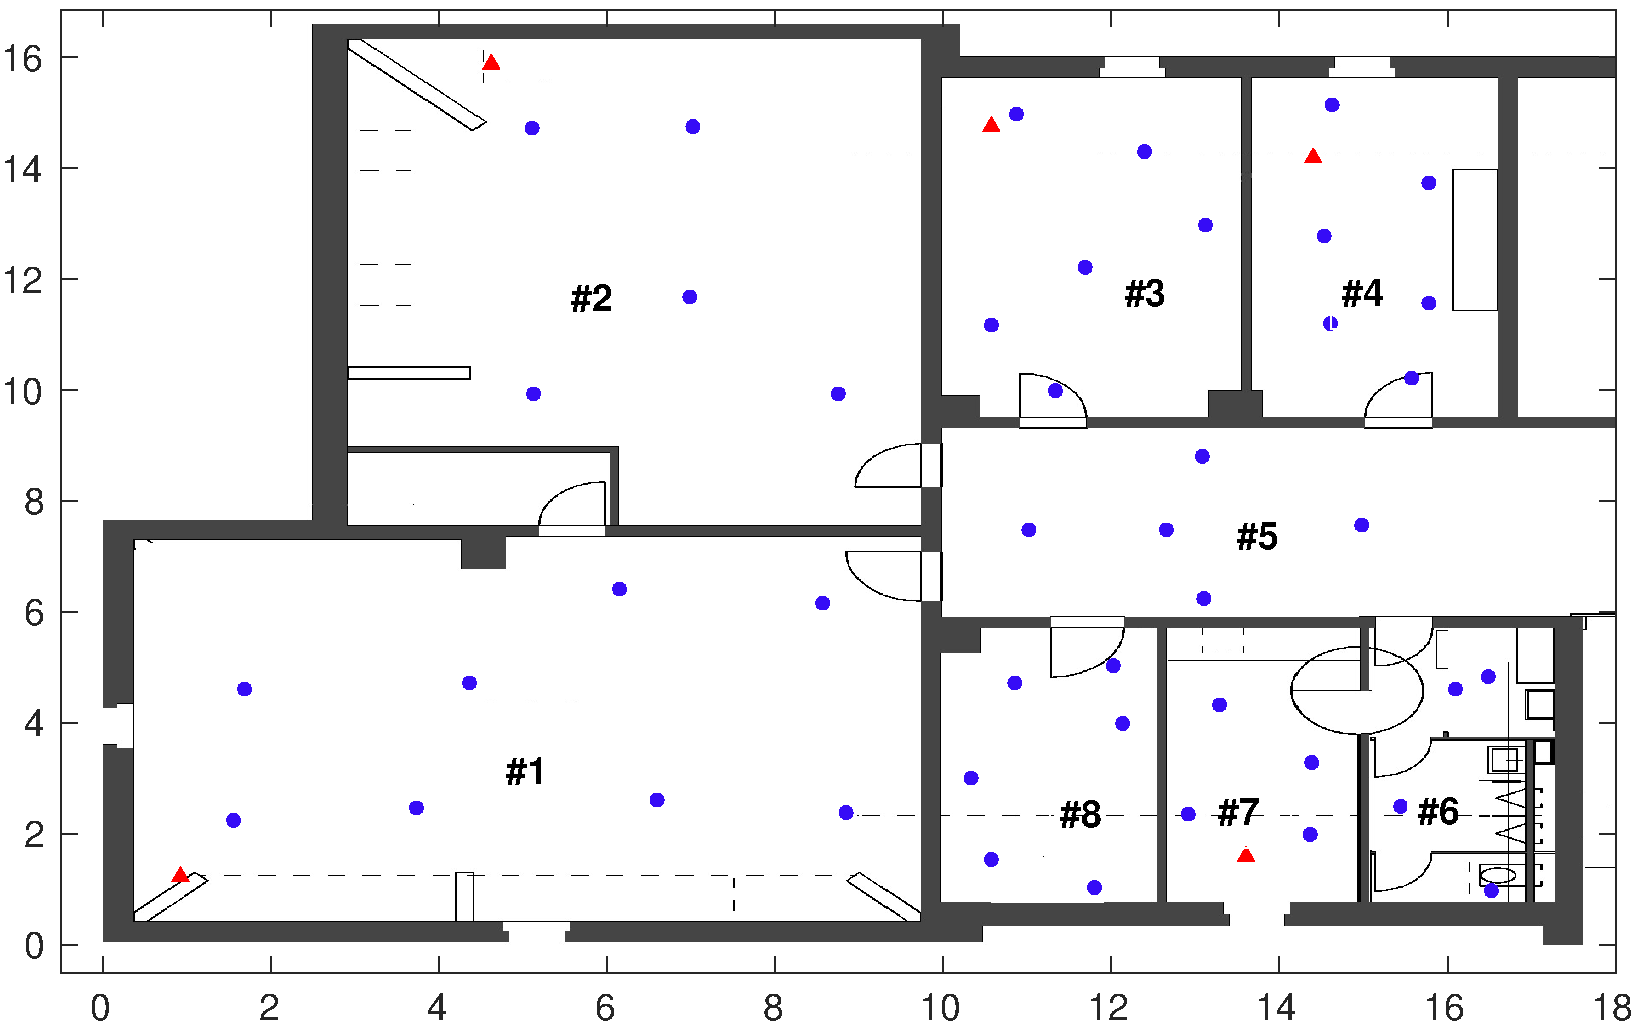
\includegraphics[width=\textwidth]{Figures/FloorPlan_ANs}
\decoRule
\caption[Floor plan]{Floor plan showing the area of interest with the anchor nodes in red, the \emph{XY}-samples in blue and the room numbers in black}
\label{fig:FloorPlanANs}
\end{figure}

The test bed was deployed on the third floor at the Institute of Computer Science (INF) of the University of Bern. The area of interest is 297m\textsuperscript{2} in size, with seven rooms connected by a large corridor. The five anchor nodes were positioned to provide maximum coverage of the area so that the mobile node is able to receive at least four of the signals at all time. The rooms were given numbers form one to eight, the corridor being also treated as a room.

\subsection{Collected Data Sets}

The samples were collected with the smartphone held approximatively one meter above the ground and always pointing in the same cardinal direction. This is important because the magnetic field measurements are influenced by the devices orientation.

The collected samples were grouped into the following data sets:

\begin{itemize}
\item \textbf{Fingerprinting data} only labeled with the room number
	\begin{itemize}
	\item Grid (223 samples)

	A set of \textbf{evenly distributed} samples gathered in a grid pattern with approximately 1.2m distance between them.
	\item Borders (373 samples)
	
	A set of \textbf{unevenly distributed} samples. The sample density is very high at the borders (walls and doors between rooms) with about one sample taken every 0.5m but only a few samples from the center of each room.
	\end{itemize}
 \item \textbf{XY data} labeled with the exact coordinates
 
 A set of 44 \textbf{evenly distributed} samples labeled with \((X,Y)\)-coordinates.
\end{itemize}

\section{Room Recognition}
\label{EvaluationRoomRecognition}

The purpose of this evaluation is to check the hypothesis that the magnetic field data improves the room recognition accuracy. Additionally we want to find out which kind of training data (evenly distributed or more samples at the borders) achieves the best results.

\paragraph{To check if the magnetic field data has a significant impact on the performance of the room recognition} 10-fold cross validation is performed on the evenly distributed \emph{Grid} data set both with and without using magnetic field data. The resulting accuracies are compared. This experiment is repeated with different SVM parameters to see if the parameters have an impact on the result. 

\paragraph{To determine the best training data set} multiple models are generated using the two training data sets (\emph{Grid}, \emph{Borders}) and different SVM parameters and kernels. The models are tested against the evenly distributed \emph{XY} data set and the resulting accuracies are compared.

The SVM parameters are either the standard pre-sets or selected with cross validation and grid search.

\subsection{Results}

Table \ref{tab:RoomRecognitionMagneticField} shows a large difference between the performance with and without magnetic field data when using cross validation. With WEKA's pre-set SVM parameters (poly-kernel, $c=1,e=1$) the improvement is very large with almost 20\%. When using the optimal parameters (determined by grid search for each case separately) the difference drops to a still significant 10\%. This drop is due to the fact that the pre-set parameters seem to be better suited to the case with magnetic field data. A comparison between the two cases using not optimal parameters is therefore unfair.

Cross validation can sometimes be a little biased. So the impact of magnetic field data was also compared by training with the \emph{Grid} data set and testing against the \emph{XY} data set, mimicking a real-world use case of the room recognition. Surprisingly this only resulted in a 2.3\% improvement.



\begin{table}
\centering
\begin{tabular}{l l l l}
\toprule
\textbf{Evaluation Type}&\textbf{with }\boldmath$B_{xyz}$&\textbf{without }\boldmath$B_{xyz}$&\textbf{Improvement} \\
\midrule
CV (pre-set)&90.1\%&70.4\%&19.7\%\\
CV (optimized)&93.3\%&83.0\%&10.3\%\\
Train: \emph{Grid}, Test: \emph{XY}&84.1\%&81.8\%&2.3\%\\
Train: \emph{Grid}, Test: \emph{XY}&97.3\%&86.8\%&10.5\%\\
\textit{(without room \#3)}&&\\
\bottomrule
\end{tabular}
\caption[Room Recognition - Magnetic Field improvements]{Accuracy of the room recognition with and without magnetic field data.}
\label{tab:RoomRecognitionMagneticField}
\end{table}

The reason for this unexpected result can be found by comparing the impact of the magnetic field data on the  room recognition accuracy for each room. We see in table \ref{tab:RoomRecognitionPerRoom} that the accuracy is improved in every room that was not already 100\%. Wit the exception of room \#3 where the accuracy drops to 0\%. 

At the time the data sets were collected room \#3 was almost empty while the two adjacent rooms contained server racks and technical equipment (near the walls separating the rooms). I expect that some of this equipment caused a disruption of the magnetic field during the time that the \emph{XY} data set was created. And therefore obscured the already weak magnetic signature of room \#3. A similar effect was observed in related work \citep{Li2012feasableMagnetic}.

When room \#3 is excluded from the test set we get the expected 10\% improvement when using magnetic field data.

\begin{table}
\centering
\begin{tabular}{l l l l}
\toprule
\textbf{Room Number}&\textbf{with }\boldmath$B_{xyz}$&\textbf{without }\boldmath$B_{xyz}$&\textbf{Improvement} \\
\midrule
\#1&100.00\%&100.00\%&-\\
\#2&100.00\%&100.00\%&-\\
\#3&0.00\%&50.00\%&-50.00\%\\
\#4&100.00\%&83.30\%&16.70\%\\
\#5&100.00\%&80.00\%&20.00\%\\
\#6&100.00\%&75.00\%&25.00\%\\
\#7&100.00\%&100.00\%&-\\
\#8&83.30\%&66.70\%&16.60\%\\
\bottomrule
\end{tabular}
\caption[Room Recognition - Accuracy per room]{Accuracy of the room recognition for each room (\emph{XY} test set, poly-kernel, optimized parameters)}
\label{tab:RoomRecognitionPerRoom}
\end{table}



Table \ref{tab:SVMconfigurationPresets} shows the accuracy for the two training data sets and two different kernel functions using WEKA's pre-set parameters. The polynomial kernel performs very well while with the RBF kernel the accuracy is below 20\% for all training data sets. The RBF kernel, with these parameters, does not seem to be a good fit for this kind of data.

With the polynomial kernel the unequally distributed \emph{Borders} data performs better. But it is only 2.3\% better than \emph{Grid}, which has 40\% fewer samples. This difference does not seem significant and is most likely due to the higher numbers of samples.

Table \ref{tab:SVMconfigurationPoly} shows the accuracy with optimal parameters for each training set and kernel. The parameters were selected with a grid search.

For both training data sets the accuracy could be slightly increased by the parameter selection, but the relative accuracy is still the same; \emph{Borders} has the highest performance with \emph{Grid} only being marginally worse.

With the optimized parameters both kernels have a similar performance, although the RBF kernels $c$ values are generally higher. A high $c$ value means that the RBF kernel's decision surface needs to be more complex to achieve the same accuracy as the polynomial kernel. It is therefore not as good at separating the samples. 

Finally to see if it is possible to train a room recognition system with a minimal number of samples the system was trained with the \emph{XY} data set and tested against the \emph{Grid}. This resulted in a accuracy of 81.2\%. This is still very high considering only 44 training samples were used.



\begin{table}

\centering
\begin{tabular}{l l l}
\toprule
\textbf{Training Data}&\textbf{Polynomial}&\textbf{RBF}\\
\textbf{(\#Samples)}&$c=1,e=1$&$c=1,g=0.01$\\
\midrule
Grid (223)&81.8\%&18.2\%\\
Borders (373)&84.1\%&11.4\%\\
\bottomrule
\end{tabular}
\caption[Room recognition - SVM pre-sets]{Accuracy of the room recognition with different training data sets using the polynomial and RBF kernel pre-sets}
\label{tab:SVMconfigurationPresets}
\end{table}

\begin{table}
\centering
\begin{tabular}{l l l l l l l}
\toprule
\textbf{Training Data}&\multicolumn{3}{c}{\textbf{Polynomial}}&\multicolumn{3}{c}{\textbf{RBF}}\\
\textbf{(\#Samples)}&\textbf{accy}&$c$&$e$&\textbf{accy}&$c$&$g$\\
\midrule
Grid (223)&84.1\%&10&1&84.1\%&100&0.01\\
Borders (373)&88.6\%&100&1&86.4\%&1000&0.01\\
\bottomrule
\end{tabular}
\caption[Room Recognition - optimized parameters]{Accuracy of the room recognition with different training data sets using the optimal parameters}
\label{tab:SVMconfigurationPoly}
\end{table}

\newpage

\section{Weighting}
\label{EvaluationWeighting}

Section \ref{EvaluationRoomRecognition} has shown that the proposed room recognition can achieve high accuracy even with a small training data set. Potentially it could be trained with the same points used to train the ranging model, eliminating the need to collect additional samples. It is now possible to evaluate the proposed weighting method and see if the information from the room recognition can be used to improve the range based localization accuracy.

In Chapter \ref{WeightingModelDefinition} a new weighting method was proposed; the \emph{Room Weights} (equation \ref{eqn: Room Weights}). The goal of this evaluation is to evaluate if the \emph{Room Weights} improve the accuracy of the trilateration and if this is true whether the accuracy can be further improved by combining the \emph{Room Weights} with the existing method of the \emph{Distance Weights}.

In a first step the new weighing method is applied with the assumption of 100\% room recognition and compared to \emph{ordinary least squares} (trilateration with no weights). This gives us a best case value for the improvements with the new weighting method.

In a second step the weighting method is applied to a real word scenario using a room recognition system trained with the the \emph{Grid} data set (accuracy of 84\%). The results are compared to the 100\% case to see how sensitive the weighing method is to errors in the room recognition.

Finally the performance of the proposed weighting method under real world conditions is compared to the \emph{Distance Weights} to see if it performs better than other simpler weighting methods.

The \emph{ranging model} and \emph{room weights} are trained with the entire \emph{XY} data set and imported into the trilateration tool. For evaluation the same data-set is used.

\subsection{Results}
In addition to the mean, standard deviation and maximum error, the results are presented as the cumulative distribution function of the localization error. This allows for a more accurate representation of the performance than just using statistical values.

\begin{table}[hb]
\centering
\begin{tabular}{l l l l l}
\toprule
\textbf{Weighting Method}&\textbf{Mean}&\textbf{STD}&\textbf{Max}&\textbf{Improv}\\
&&\textbf{}&\textbf{Error}&\textbf{over OLS}\\
\midrule
OLS&2.74m&1.57m&8.25m&\\
Room Weights (100\%)&2.35m&1.22m&4.89m&14.2\%\\
Room+Distance Weights (100\%)&2.29m&1.16m&4.65m&16.4\%\\
Room+Distance Weights (84.1\%)&2.40m&1.25m&5.69m&12.4\%\\
Distance Weights&2.42m&1.19m&5.37m&11.3\%\\
\bottomrule
\end{tabular}
\caption[Weighting - statistical values]{Comparison of the statistical values for the different weighting methods}
\label{tab:WeightingStatisticalValues}
\end{table}

\begin{figure}[p]
\centering
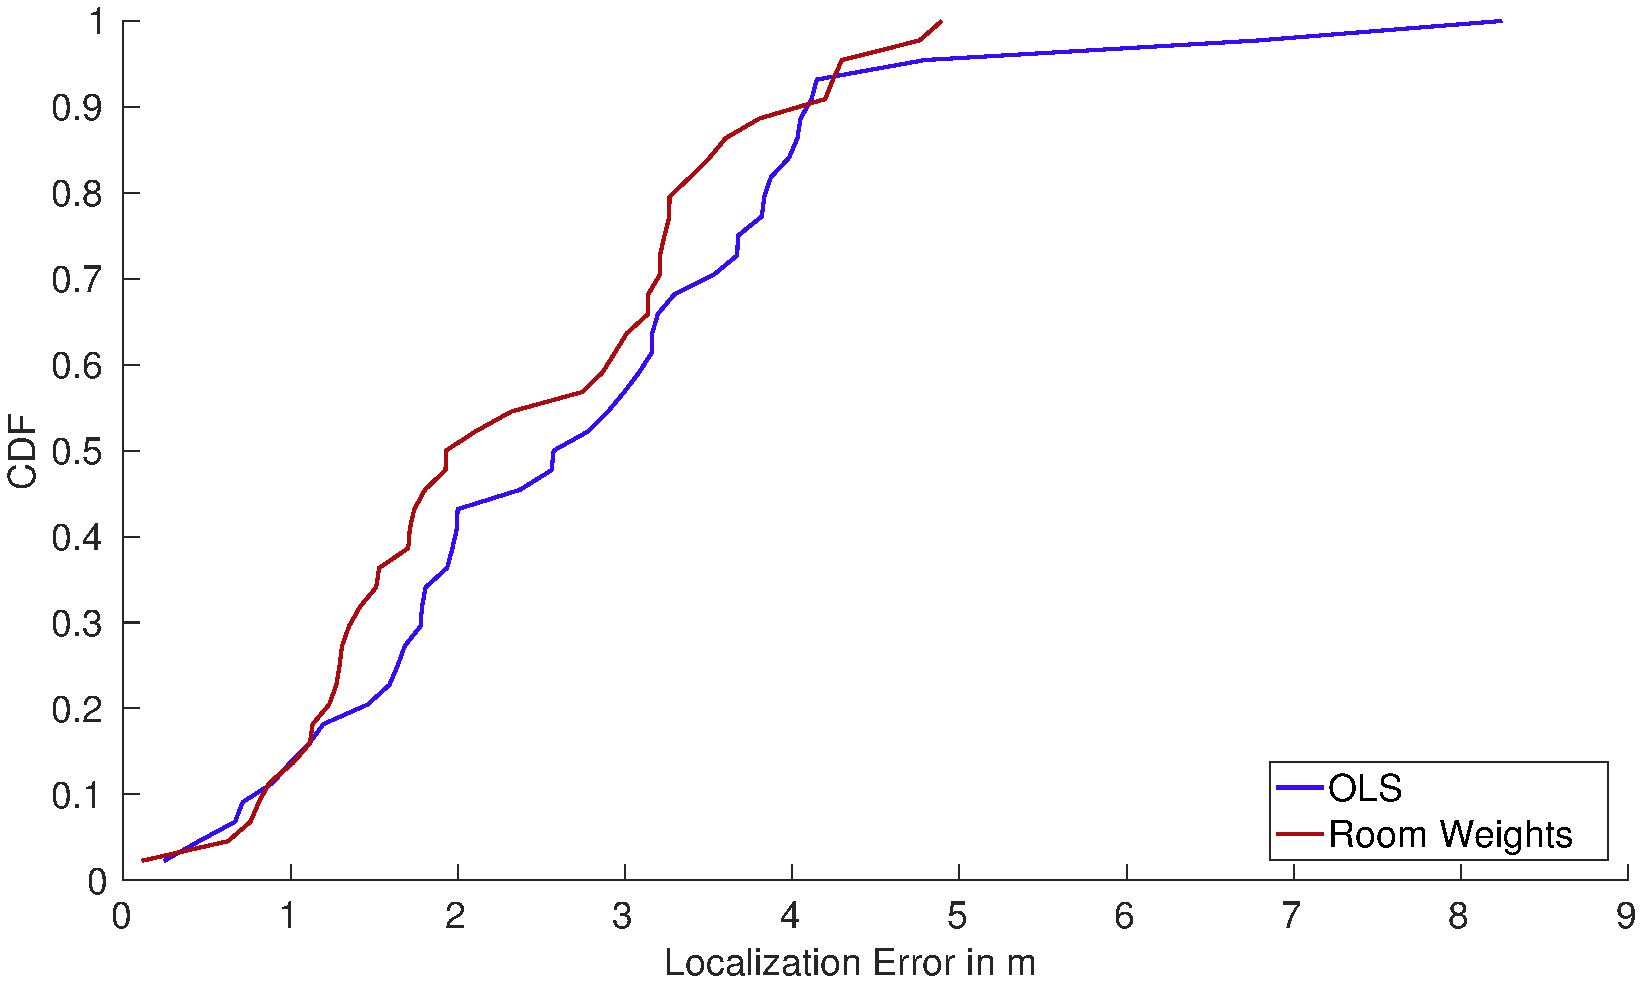
\includegraphics[width=\textwidth]{Figures/WeightingCDF_RW}
\decoRule
\caption[CDF Room Weights method (best-case)]{The Localization error with the \emph{Room Weights}.}
\label{fig:WeightingCDFRoom}
\end{figure}

\begin{figure}[p]
\centering
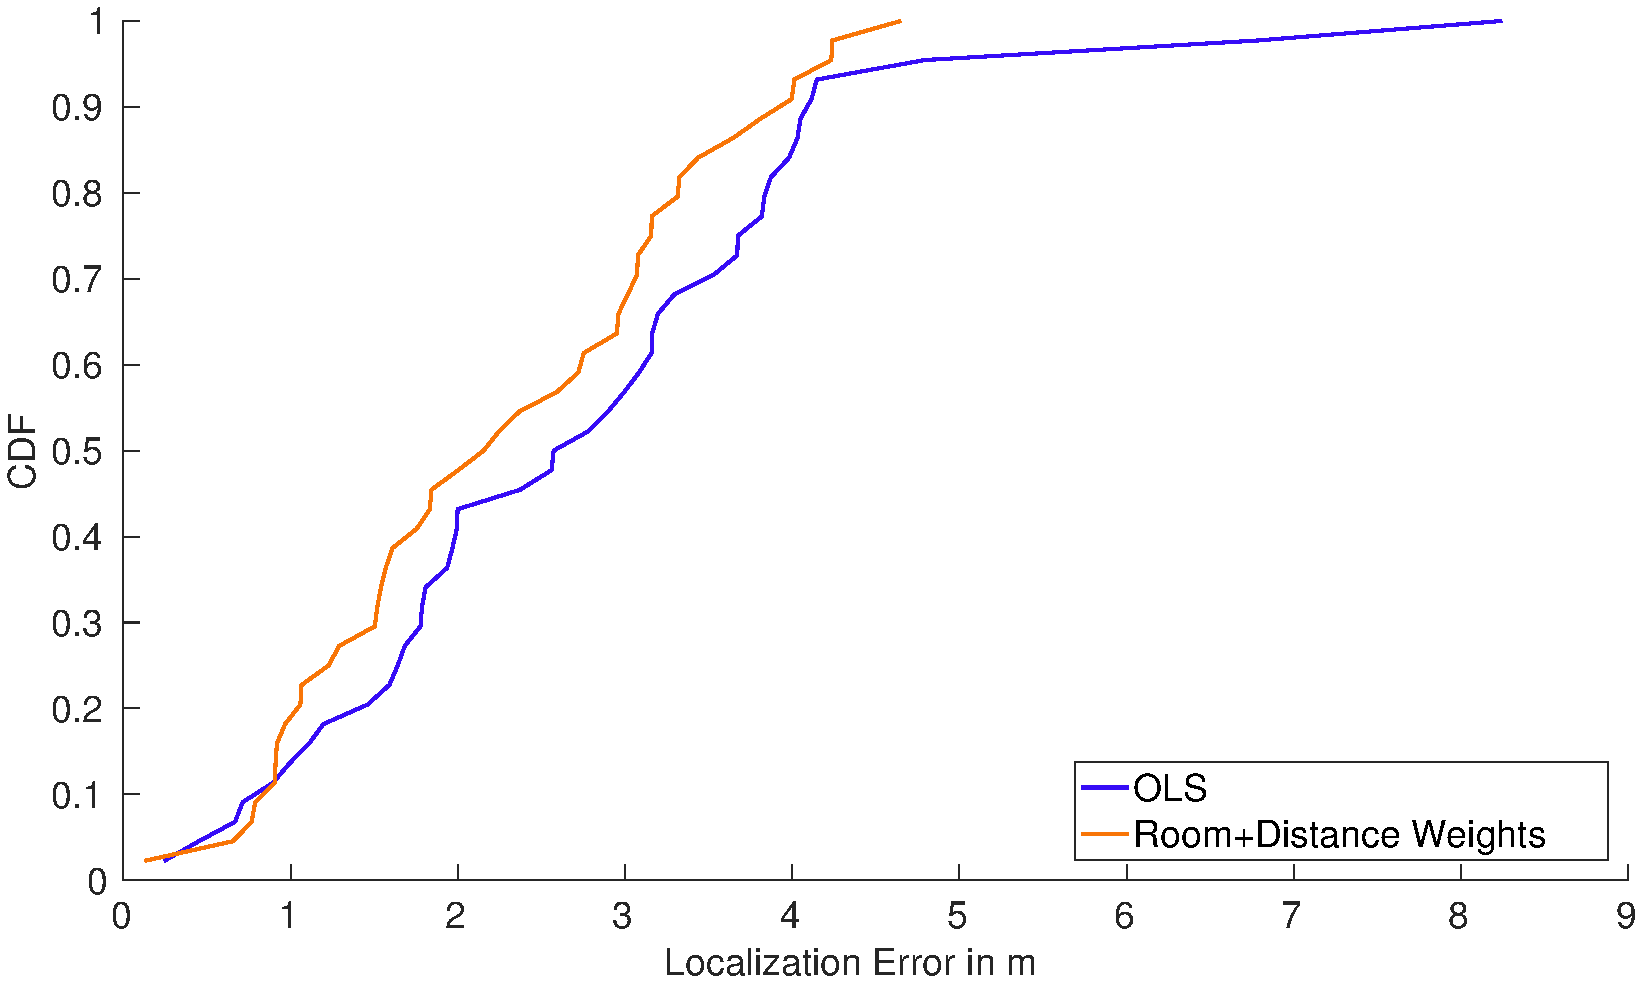
\includegraphics[width=\textwidth]{Figures/WeightingCDF_RDW}
\decoRule
\caption[CDF Room+Distance Weights method (best-case)]{The Localization error with the \emph{combined room and distance weights}.}
\label{fig:WeightingCDFRoomDistance}
\end{figure}

The results with 100\% room recognition show a improvement of the \emph{Room Weights} over \emph{OLS}. The mean error is 14.2\% ($\approx$0.4m) lower, the standard deviation smaller and the maximum error was reduced by $\approx$3.4m. But when looking at the CDF plot (figure: \ref{fig:WeightingCDFRoom}) the improvement, although visible, does not seem very dramatic and is mainly due to the large reduction in the maximum error.

The results also show that combining the \emph{Room} and \emph{Distance Weights} does indeed yield a further small improvement. While the mean error is only marginally increased, it lowers the maximum error even further and smooths out the CDF curve (figure: \ref{fig:WeightingCDFRoomDistance}).

The comparison between the performance of the weighting in a best case scenario and real world case, shows that there is indeed a error introduced by the room recognition. But the CDF (figure: \ref{fig:WeightingCDFrealRoom}) shows that this error is overall very small and mainly due to a few samples with a large error, which increase the maximum error.

However when taking into account this error, the real world performance of the proposed weighting method is almost the same as the existing simpler \emph{Distance Weights}. This is apparent in figure \ref{fig:WeightingCDFrealDistance}. The mean error is only a few centimeters lower (0.07m) and the maximum error even higher than with the \emph{Distance Weights}.

\begin{figure}[bh]
\centering
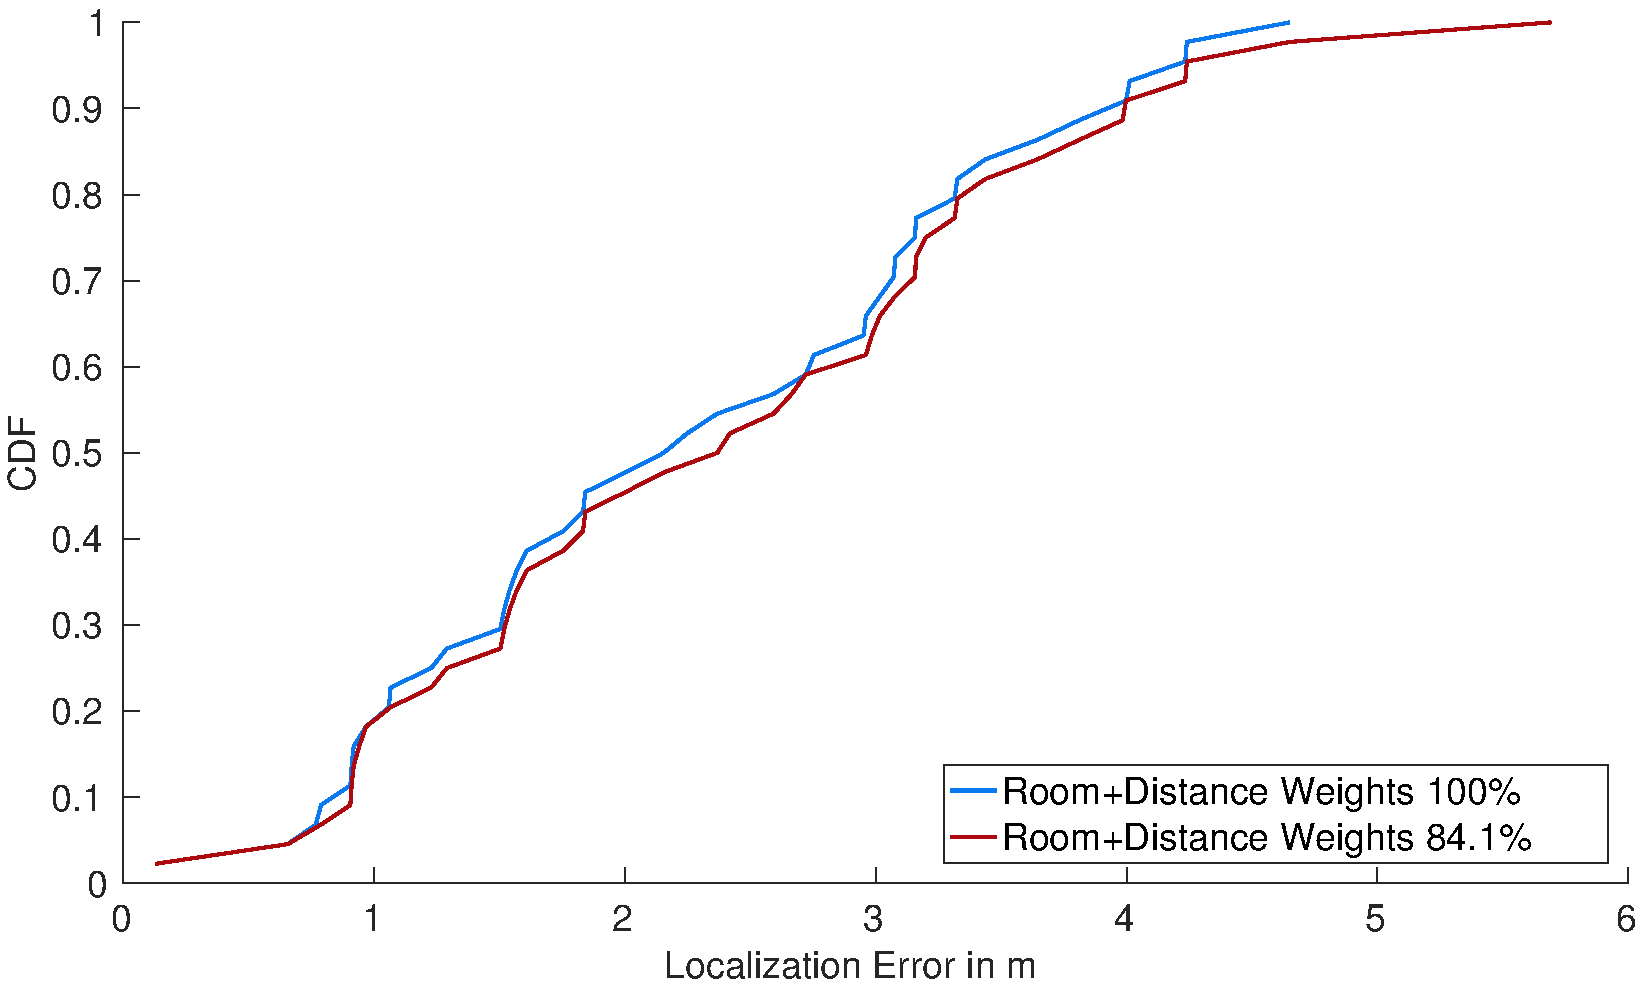
\includegraphics[width=\textwidth]{Figures/WeightingCDF_realRW}
\decoRule
\caption[CDF Room+Distance Weights - best-case/real world comparison]{Localization error with \emph{combined room and distance weights} in a best-case and real world scenario}
\label{fig:WeightingCDFrealRoom}
\end{figure}

\begin{figure}
\centering
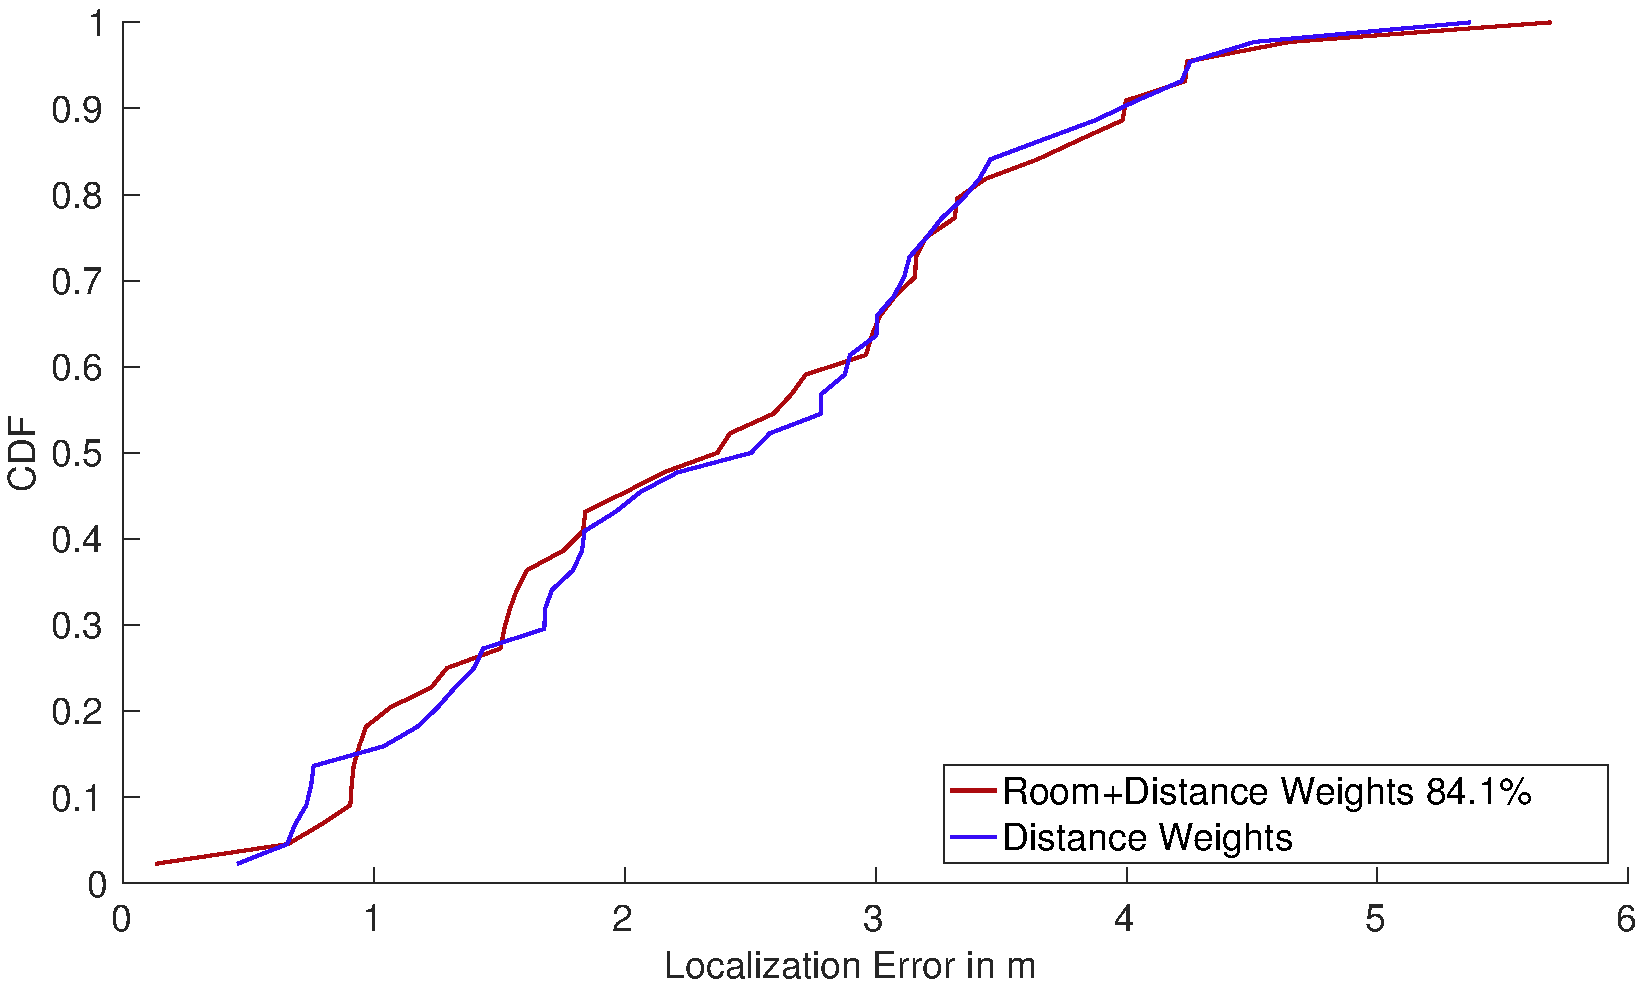
\includegraphics[width=\textwidth]{Figures/WeightingCDF_realDistance}
\decoRule
\caption[CDF Room+Distance Weights - comparison against Distance Weights]{Localization error for the \emph{combined room and distance weights} and \emph{Distance Weights}}
\label{fig:WeightingCDFrealDistance}
\end{figure}